\section{Methods and Materials}

When testing navigation functions for the H.A.C.K robot, Webots (version R2020b rev. 1) is used as a simulation tool~\cite{Webots}. Webots has a physics engine with build-in fluid dynamics parameters, which is useful to emulate the forces, such as water resistance, acting on the robot when moving through water~\cite{WebotsRef}.

Webots have different parameters that were set and can be found here:\cite{ProjectGithub}


Furthermore, it supports a variety of sensors~\cite{WebotsRef}, easing the implementation and testing of the different navigation functions. For the noise on the beacon based position, is Gaussian with a standard deviation of 1.02 meter.\\
%\todo[inline]{Niko: add noise stuff here}

Three different navigation functions are implemented, with different sensor implementations. \textit{The random walk} ( \ref{section:rng_walk} ) requires a border detection system, to ensure it doesn't fall of an edge. \textit{The boundary-based navigation function}, needs to know the boundaries of the workspace and its position relative to them. And \textit{the Slicer algorithm} requires a detailed scan of the work-surface as the navigation function requires a detailed map of the work-surface dimensions. This algorithm also uses beacons to localise itself inside this map.

Webots is compatible with the Robot Operating System (ROS), which eases the management of inter-process communication between different nodes running simultaneously~\cite{WebotsRef}~\cite{ROSTech}.

\begin{figure}[ht]
    \captionsetup{justification=centering}
    \centering
    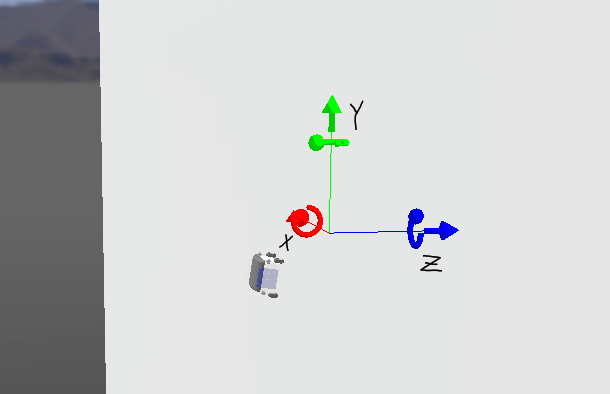
\includegraphics[width=0.4\textwidth]{Figures/rob_fig.png}
    \caption{One of the testing worlds the algorithms are tested on. Here, it is a flat plane of $100x42m$.}
    \label{fig:example_test_world}
\end{figure}

In figure~\ref{fig:example_test_world}, an example of the plane world the algorithms are tested on is visualized. The research on different ship-hulls was initially done, but resulted in complexities while simulating the interactions of the robot with the ship-hull. As it was observed that the surface on where the robot stands could be approximated to be a plane, relative to the robot, and could be used as a testing environment for the different algorithms.
%, so different generalised simple geometric figures could be used for testing the robot in Webots, to see how the algorithms operated on different world setups.

\subsection{Navigation Algorithm: Random Walk Path Planner}\label{section:rng_walk}

The general functionality of a random walk path plan is to make the robot move to a randomly generated point in the environment without any knowledge of the global map. The robot will move until this point is reached, then global planer will calculate a new random point. The local planner generates a heading based on the point from the global planner and the robot will move according to this heading. The robot will continue to move according to the heading generated by the local path planner until receiving a sensor input indicating an obstacle or the goal point is reached and the navigation function in the global planner will calculate a new point again. The implementation algorithm can be seen in figure~\ref{algo:RndWalk}.

\begin{algorithm}
	\caption{Random Walk} \label{algo:RndWalk}
	
    \small
	\begin{algorithmic}[1]
		\If {$hull \;!=\; clean$}
			\If {$point visited = true$}
				\State Generate a new point ({x,y}) at r dist from HACK and send it to the local-planner.
			\Else
			    \State Resend old point (x,y) to local planner.
			\EndIf
		\EndIf
	\end{algorithmic} 
\end{algorithm}

%\begin{algorithm}
    \begin{small}
	\caption{Time-Dependent Random Walk}\label{algo:AugRndWalk}
	\begin{algorithmic}[1]
		\If {$hull \;!=\; clean$}
		    \State timeToPass = time + randomNumber.
			\If {$point visited = true\;||\;timeToPass < timeNow $}
			   \State Generate a new point ({x,y}) at r dist from HACK and send it to the local-planner.
		    \Else
			    \State Resend old point ({x,y}) to local-planner.
			\EndIf	
		\EndIf
	\end{algorithmic} 
	\end{small}
\end{algorithm}

%\subsection{Navigation Algorithm: time-dependent Random Walk Path Planner}

%The time-dependent random-walk has an added element to the non-augmented one. Here, the path planner will at random times change goal position during transit, which is not based on a sensor input, but on time. This time is used to insure that H.A.C.K does not get stuck, trying to reach the point. The implementation of this algorithm can be seen, in algorithm \ref{algo:AugRndWalk}.

\subsection{Navigation Algorithm: Boundary-based Algorithm }% Ola's algorithm

\textbf{Requirement for this algorithms:} Beacons with GPS modules mounted on critical points of the hull, indicating boundaries.

\textbf{Sensors used:} IMU, Beacon-Based Localisation 

This navigation function uses the beacons as boundaries that limit the work-space of H.A.C.K., which eases the implementation of a full coverage system on non-planar shapes. The algorithm moves along a height layer until it completes a pass, then it goes down a height layer and completes a pass, this continues until it has reached the bottom of the shape, then the robot will reset the pose to the start pose on the other side of the shape. This process is visualised in figure~\ref{fig:globalplannerthatolamadehihi}. The pseudo code for this algorithm can be seen here \ref{alg:BBA} 

\begin{figure}[ht]
    \captionsetup{justification=centering}
    \centering
    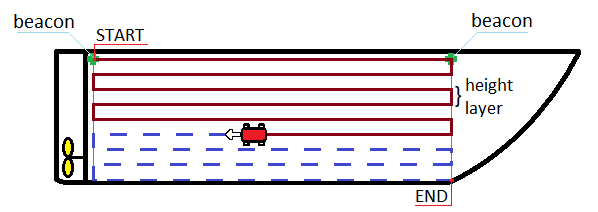
\includegraphics[width=0.5\textwidth]{Figures/comparison/boat.png}
    \caption{How the Beacon-based Algorithm generates the path for the robot and how the beacons are placed.}
    \label{fig:globalplannerthatolamadehihi}
\end{figure}

\begin{algorithm}
    \begin{small}
	\caption{Boundary-based Algorithm}\label{algo:BBA}
	\small
	\begin{algorithmic}[1]
		\If {surface\_boundary != True and stern\_boundary != True and start == False}
		    \State start = True
		\EndIf
		\If {start == True}
		    \State move towards the bow boundary
        		\If {stern\_boundary == True or bow\_boundary == True}
        		    \State move down a height layer
        		\EndIf
        		\If {keel\_boundary == True}
        		    \State go to the other side of the boat
        		    \State start = False
			    \EndIf	
		\EndIf
	\end{algorithmic}
	\label{alg:BBA}
	\end{small}
\end{algorithm}

\subsection{Navigation Algorithm: Slicer Path Planner}

\textbf{Requirement for this algorithms:} Full-scan of the ship's hull. The scan needs to be processed before use in this algorithm.

\textbf{Sensors used:} GPS, Sonar scan
The path planning has the ability to do a full coverage, of the ship hull, with minimal path overlap. This is possible due to a complete, known global map, derived from the ship model. The robot is using beacons as in the beacon-based method, to localise itself. The tool-path is derived in the same manner, as a Slicer program derives a path for a 3D printer. The path is generated on the global map. The implementation for this method is presented in algorithm~\ref{algo:CompCove}. This algorithm and the BBA, would produce a similar path, to distinguish them the Slicer algorithm derives a vertical path, where the BBA produces a horizontal path.

\begin{algorithm}
	\caption{Slicer coverage} \label{algo:CompCove}
	\begin{small}
	
	
	\begin{algorithmic}[1]
		\State Load $STL$ 
		\State Slice $STL$ into separate layers
		\For{$Point$ in Slice}
		\State Store Slice (x,z) and layerHeight(y) in a List
		\EndFor
		\State idx = 0
		\If {$idx\;!= length\;of\;List$}
		    \State x,y,z = List[idx]
		    \State send (x,y,z) to local planner
		    \State idx++
		\Else
		\State Hull is clean
		\EndIf
	\end{algorithmic}
	\end{small}
\end{algorithm}


\subsection{Planners}
\noindent
\textbf{Global: }Each navigation functions is implemented in the global planner. The navigation function is used to, derive the new goal position for H.A.C.K the robot.The global planner is updated at frequency 5 Hz, to reduce the computational power.\\
\textbf{Local: } For each new goal point the global planner sends to the global planner, the local planner calculates a new heading for H.A.C.K the robot. The local planner is update at a frequency of 50 Hz, to maintain a heading for H.A.C.K so it does not drift of course.


\subsection{System overview}
The robot shown in fig. \ref{fig:example_test_world} is a conceptual simulation of differential drive robot designed to enable it to stick to the boat with a constant pressure. Multiple algorithms are tested on several geometric figures, imitating different ship-hull features. 


The sensors that are available without modifications are IMU, pressure sensor and two monocular cameras.

%System that the algorithms were simulated on
%% Nicolai will fill this out or provide a list





%\textit{\textcolor{gray}{What we did: \begin{itemize}
%    \item assumptions and prior art
%    \item theory, models, basic equations
%    \item block diagrams
%    \item descriptions of data collection methods
%    \item algorithms
%\end{itemize}}}

%\textit{\textcolor{gray}{Remember to not mix methods and results, also avoid referring to specific hardware, quantities etc (to the extent possible). }}

